\documentclass[11pt]{article}
\usepackage[utf8]{inputenc}
\usepackage[T1]{fontenc} % uses T1 fonts (better quality)
\usepackage{mathptmx} % uses Times fonts
% \usepackage{lmodern} % uses Latin Modern fonts
\usepackage{pdfpages}
% \usepackage[table,xcdraw,dvipsnames]{xcolor}
\usepackage[margin=1in]{geometry}
\usepackage{graphicx}
\graphicspath{ {./graphics/} }
% \usepackage{nopageno} % no page numbers
\usepackage{bm}
\usepackage{booktabs}   % for table borders
\usepackage{float}
\usepackage{gensymb}
\usepackage[shortlabels]{enumitem}
\usepackage[makeroom]{cancel}

\begin{document}
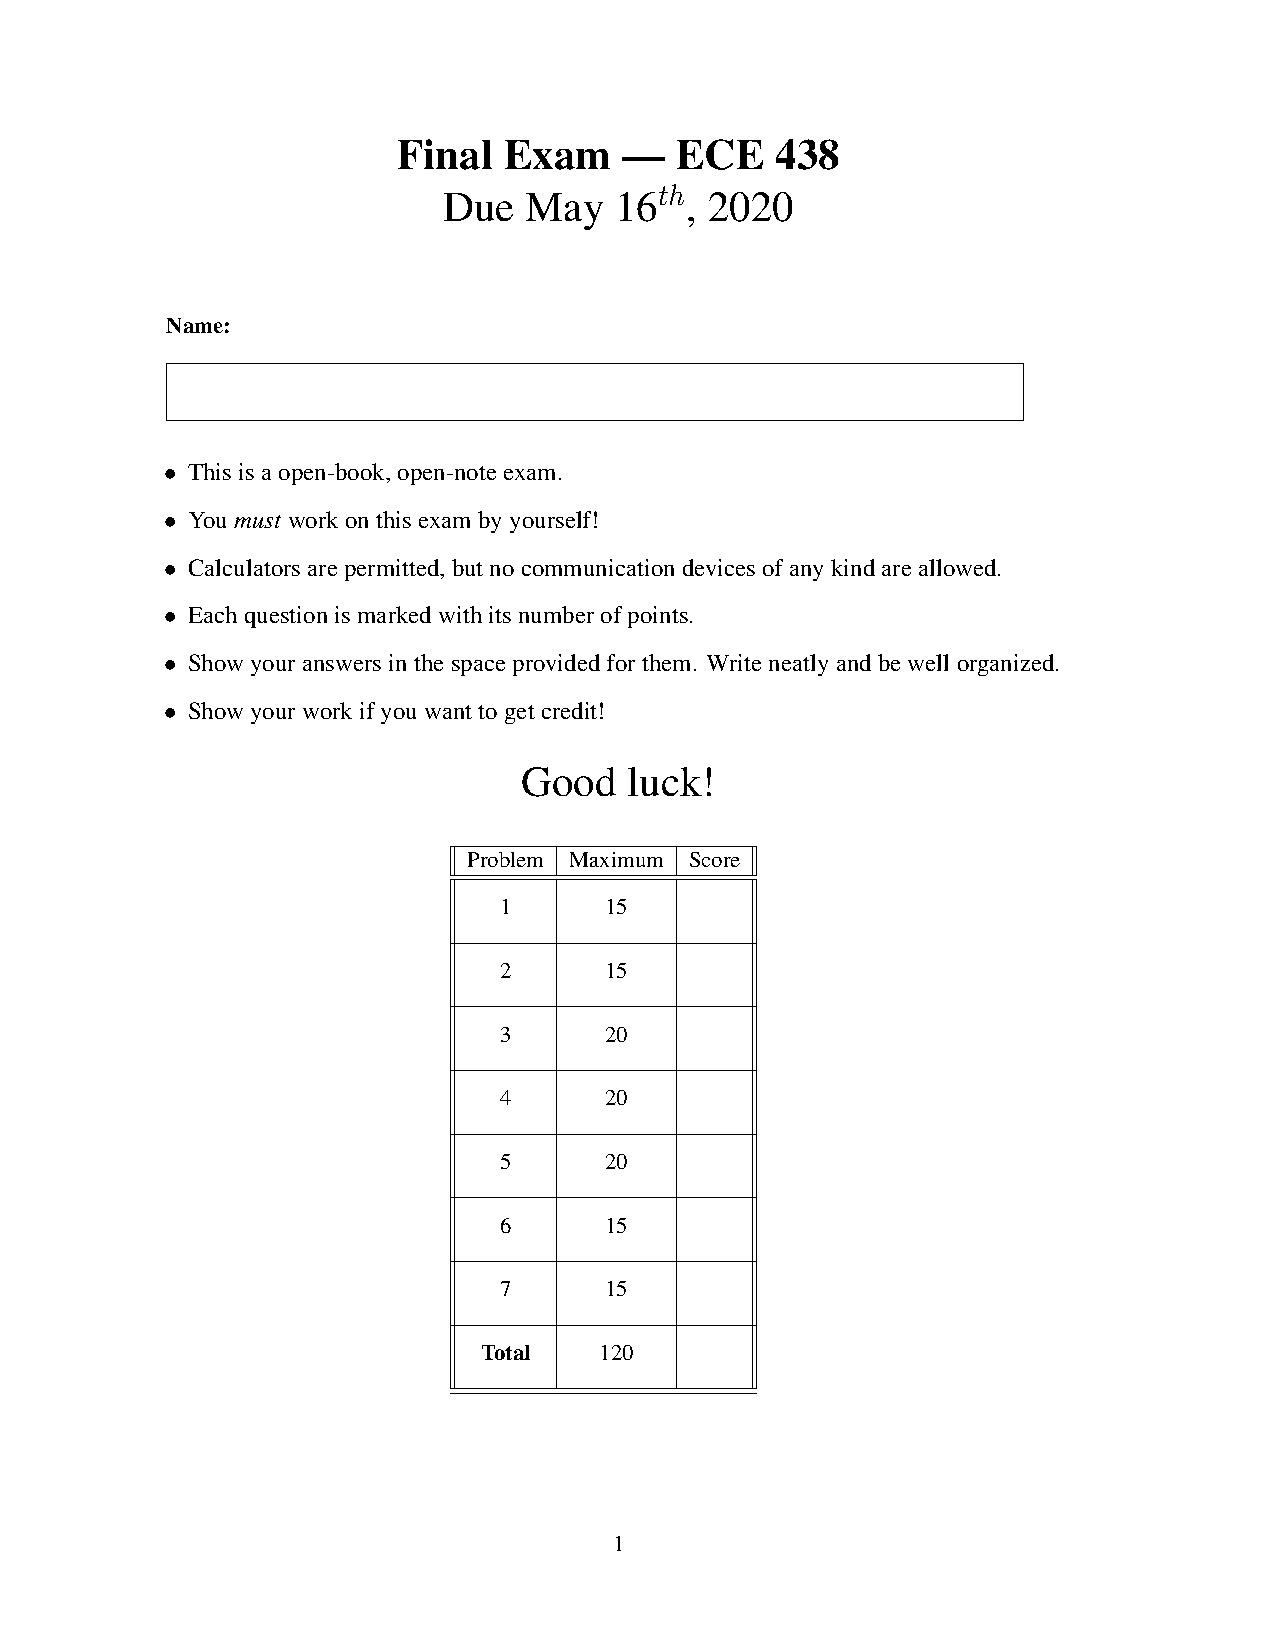
\includepdf[pages=1]{Final.pdf}
\begin{enumerate}
    \item \textbf{(15 points)} You are looking to accelerate public-key encryption and found through simulation that 95\% of the execution time of a particular algorithm is spent performing modular multiplication. Assume for the following problems that the execution time of your algorithm is 2 seconds without hardware acceleration.
    \begin{enumerate}
        \item What would be the minimum achievable execution time of this same algorithm if you developed hardware that could accelerate just the modular multiplication by 50x? Calculate the overall speedup.\\[1em]
        $\mathrm{t_{new}=}$\resizebox{4em}{!}{$\ \frac{2\mathrm{s}\times 0.95}{50\mathrm{x}}$}$+2\mathrm{s}\times (1-0.95)=0.138\mathrm{s}$\\[0.25em]
        Speedup$\ =$\resizebox{6.5em}{!}{$\ \frac{1}{\frac{0.95}{50\mathrm{x}}+(1-0.95)}$}$\ =14.493$x\\

        \item What would be the execution time and speedup achievable with a 20x acceleration of modular multiply?\\[1em]
        $\mathrm{t_{new}=}$\resizebox{4em}{!}{$\ \frac{2\mathrm{s}\times 0.95}{20\mathrm{x}}$}$+2\mathrm{s}\times (1-0.95)=0.195\mathrm{s}$\\[0.25em]
        Speedup$\ =$\resizebox{6.5em}{!}{$\ \frac{1}{\frac{0.95}{20\mathrm{x}}+(1-0.95)}$}$\ =10.256$x\\

        \item What is the name given to the design principle used in parts a) and b)?\\[1em]
        Amdahl's Law\\

        \item What would the theoretical maximum speedup be for your program if you could infinitely accelerate modular multiply?\\[1em]
        $\mathrm{t_{new}=}$\resizebox{5em}{!}{$\ \cancelto{0}{\frac{2\mathrm{s}\times 0.95}{\infty}}$}$+2\mathrm{s}\times (1-0.95)=0.1\mathrm{s}$\\[0.25em]
        Speedup$\ =$\resizebox{2em}{!}{$\frac{2\mathrm{s}}{0.1\mathrm{s}}$}$\ =20$x\\
    \end{enumerate}
\newpage
    \item \textbf{(15 points)} Imagine you have a 1GHz RISC processor with split L1 instruction and data caches, each 16kB in size with a hit time of 1ns. Access to main memory takes 50 ns, and 35\% of instructions access memory. The L1 instruction cache miss rate is 1\%, while the L1 data cache miss rate is 4\%.
    \begin{enumerate}
        \item Calculate the Average Memory Access Time (AMAT) for each of the L1 caches.\\[1em]
        $\mathrm{AMAT_{I\$}=1ns+0.01\times 50ns=1.5ns}$\\[0.25em]
        $\mathrm{AMAT_{D\$}=1ns+0.04\times 50ns=3ns}$\\

        \item Assuming your processor has a CPI of 1.3 with an ideal memory hierarchy, what is the CPI considering memory stalls?\\[1em]
        $\mathrm{CPI=1.3\frac{cc}{instr}+0.01\times 50\frac{cc}{instr}+0.04\times 0.35\times 50\frac{cc}{instr}=2.5\frac{cc}{instr}}$\\

        \item You are considering the inclusion of a 256kB L2 cache to improve your performance. If the miss rate of the L2 is 35\%, what would the AMAT of the L1 instruction and data caches be with the L2 cache? Assume a 6ns L2 hit time.\\[1em]
        $\mathrm{AMAT_{L2}=6ns+0.35\times 50ns=23.5ns=23.5cc}$\\[0.25em]
        $\mathrm{\qquad AMAT_{L2}}$ is the new miss penalty of the L1 caches.\\[0.25em]
        $\mathrm{AMAT_{I\$}=1ns+0.01\times 23.5ns=1.235ns}$\\[0.25em]
        $\mathrm{AMAT_{D\$}=1ns+0.04\times 23.5ns=1.94ns}$\\

        \item What would the CPI of your processor be with the L2 cache? What is the speedup due to the L2 cache?\\[1em]
        $\mathrm{CPI=1.3\frac{cc}{instr}+0.01\times 23.5\frac{cc}{instr}+0.04\times 0.35\times 23.5\frac{cc}{instr}=1.864\frac{cc}{instr}}$\\[0.25em]
        Speedup$\ =\frac{2.5}{1.864}=1.3412$x\\
    \end{enumerate}
\newpage
    \item \textbf{(20 points)} For the following problem, assume a 5-stage pipelined processor with a branch delay slot and branch resolution in the Execute stage. Consider the code below:
\begin{verbatim}
    addi $t2, $t1, 48
loop:
    lw $t4, 40 ($t1)
    lw $t5, 80 ($t1)
    add $t6, $t4, $t5
    sw $t6, 120 ($t1)
    bne $t1, $t2, loop
    addi $t1, $t1, 4
    add $t2, $t1, $t3
\end{verbatim}
    \begin{enumerate}
        \item Draw the pipeline execution diagram for the first \textit{two} iterations of the above code when an “assume not taken” branching scheme is used.
\begin{table}[ht]
\centering
\resizebox{\textwidth}{!}{%
\begin{tabular}{@{}l|llllllllllllllllllll@{}}
Clock cycle        & 1 & 2 & 3 & 4 & 5 & 6 & 7 & 8 & 9 & 10 & 11 & 12 & 13 & 14 & 15 & 16 & 17 & 18 & 19 & 20 \\ \hline
\texttt{addi \$t2, \$t1, 48}  & F & D & E & M & W &   &   &   &   &    &    &    &    &    &    &    &    &    &    &    \\
\texttt{lw \$t4, 40 (\$t1)}   &   & F & D & E & M & W &   &   &   &    &    &    &    &    &    &    &    &    &    &    \\
\texttt{lw \$t5, 80 (\$t1)}   &   &   & F & D & E & M & W &   &   &    &    &    &    &    &    &    &    &    &    &    \\
\texttt{add \$t6, \$t4, \$t5}  &   &   &   & F & {\color[HTML]{FE0000}D} & D & E & M & W &    &    &    &    &    &    &    &    &    &    &    \\
\texttt{sw \$t6, 120 (\$t1)}  &   &   &   &   & F & F & D & E & M & W  &    &    &    &    &    &    &    &    &    &    \\
\texttt{bne \$t1, \$t2, loop} &   &   &   &   &   &   & F & D & E & M  & W  &    &    &    &    &    &    &    &    &    \\
\texttt{addi \$t1, \$t1, 4}   &   &   &   &   &   &   &   & F & D & E  & M  & W  &    &    &    &    &    &    &    &    \\
\texttt{lw \$t4, 40 (\$t1)}   &   &   &   &   &   &   &   &   & {\color[HTML]{FE0000}X} & F  & D  & E  & M  & W  &    &    &    &    &    &    \\
\texttt{lw \$t5, 80 (\$t1)}   &   &   &   &   &   &   &   &   &   &    & F  & D  & E  & M  & W  &    &    &    &    &    \\
\texttt{add \$t6, \$t4, \$t5}  &   &   &   &   &   &   &   &   &   &    &    & F  & {\color[HTML]{FE0000}D}  & D  & E  & M  & W  &    &    &    \\
\texttt{sw \$t6, 120 (\$t1)}  &   &   &   &   &   &   &   &   &   &    &    &    & F  & F  & D  & E  & M  & W  &    &    \\
\texttt{bne \$t1, \$t2, loop} &   &   &   &   &   &   &   &   &   &    &    &    &    &    & F  & D  & E  & M  & W  &    \\
\texttt{addi \$t1, \$t1, 4}   &   &   &   &   &   &   &   &   &   &    &    &    &    &    &    & F  & D  & E  & M  & W
\end{tabular}%
}
\end{table}
        \item How many clock cycles are required to execute the above code to \underline{completion} when an “assume not taken” branching scheme is used?\\[1em]
        We have one cycle for the first \texttt{addi}. Then we have eleven loop iterations in which the \texttt{bne} is “Taken,” each requiring eight cycles (see diagram above). Then we have the last loop iteration in which the \texttt{bne} is “Not Taken,” requiring seven cycles (no flushing). We then have four cycles to drain the pipeline (i.e. to finish the \texttt{bne}) and finally one cycle to complete the last \texttt{add} instruction. Therefore, the number of clock cycles required is:\\
        $1+11\times 8+7+4+1=101$ clock cycles.\\

        \item How many clock cycles are required to execute the above code assuming a 100\% correct branch predictor.\\[1em]
        A 100\% correct branch predictor means no flushes, therefore, the number of clock cycles required is:\\
        $1+12\times 7+4+1=90$ clock cycles.\\
\newpage
        \begin{figure}[h!]
        \centering
        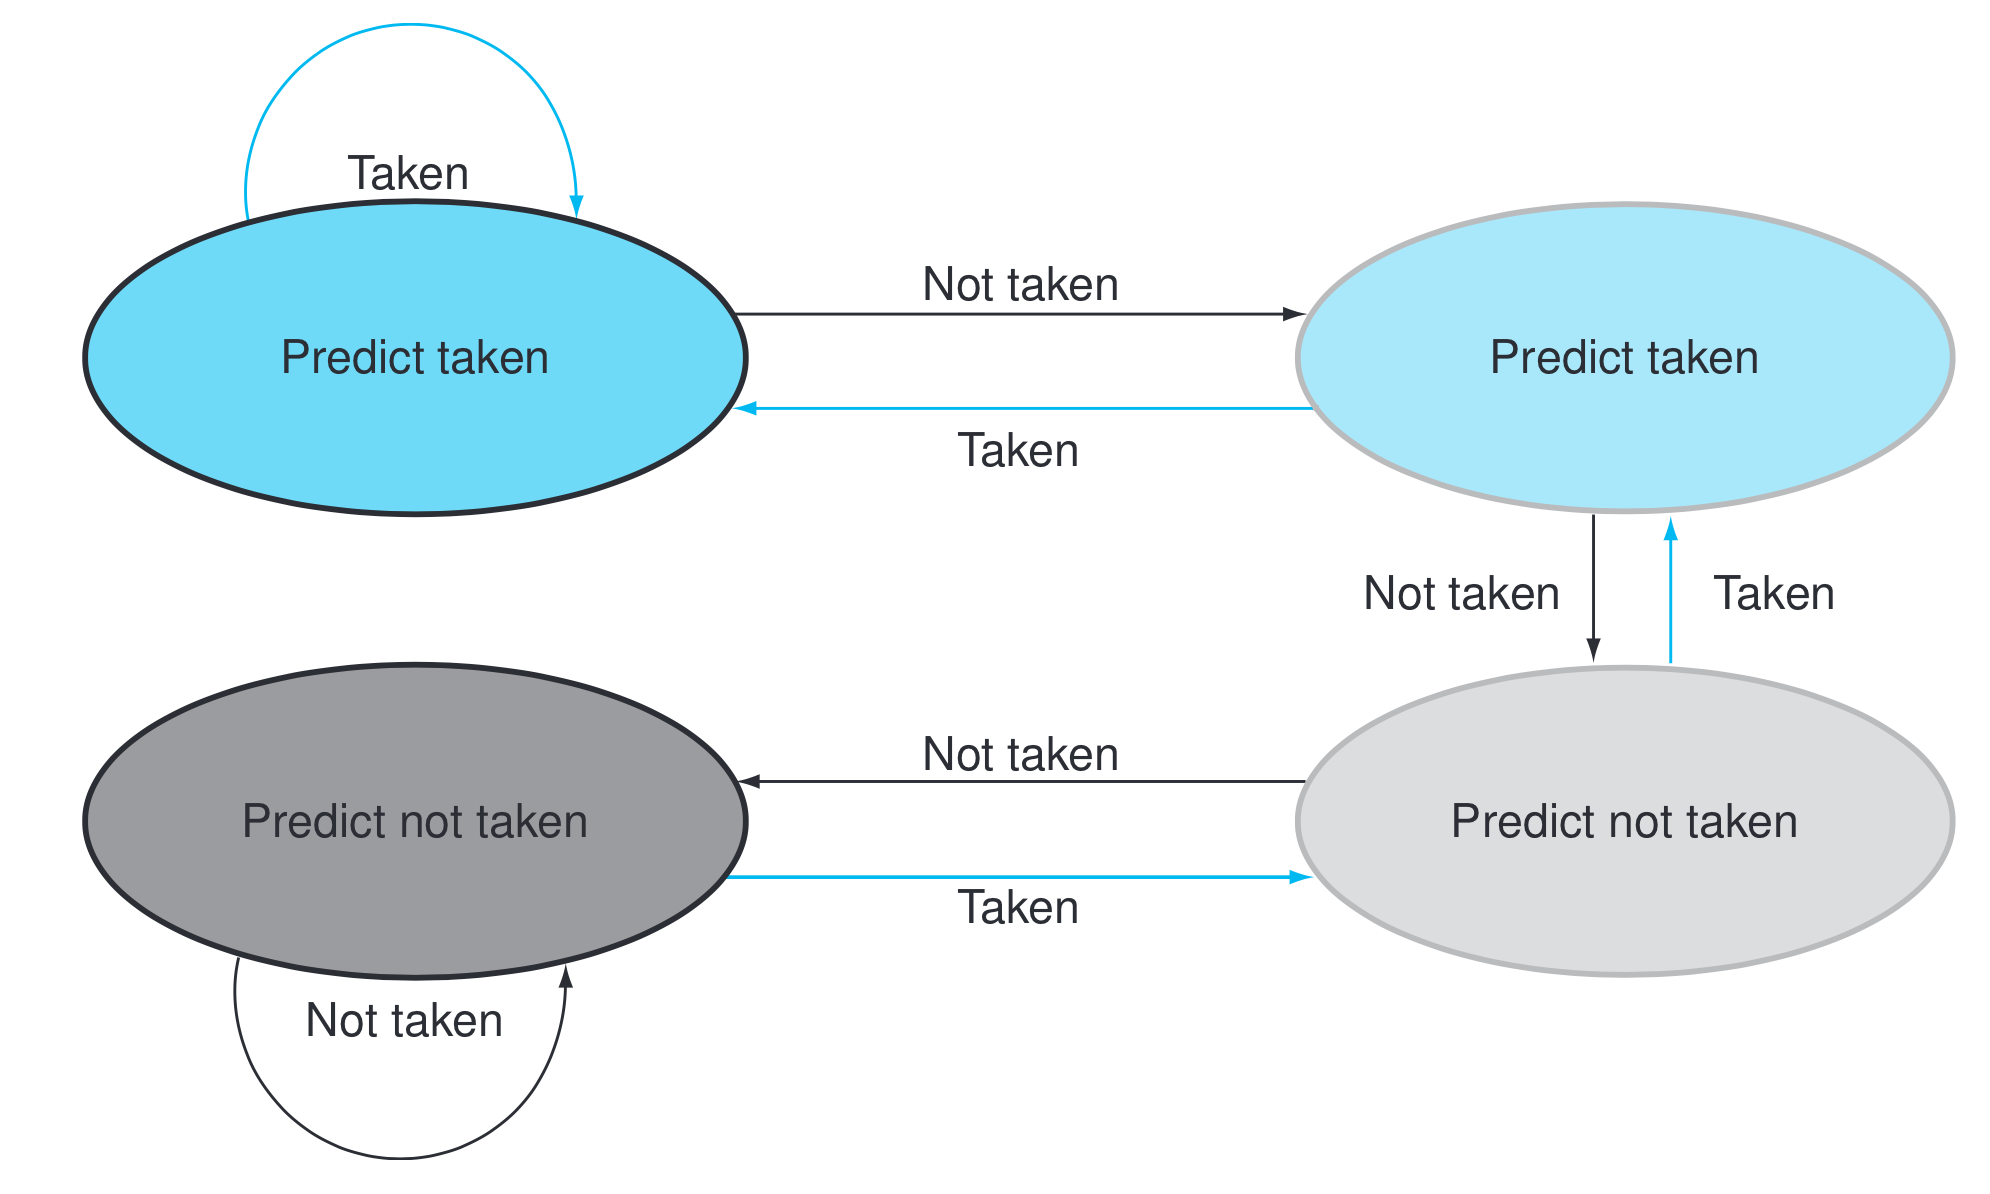
\includegraphics[width=0.80\textwidth]{Screen Shot 2020-05-14 at 21.35.45.png}
        % \caption{}
        % \label{fig:I2Cdemo}
        \end{figure}
        \item Consider the use of the two-bit predictor shown above. Assuming the predictor starts in the bottom right state (\textit{different than homework}), how many clock cycles are required to execute the above code?\\[1em]
        If the predictor is in the bottom right state (weakly Not Taken) when entering the loop, it will predict not taken for the first execution of \texttt{bne} which will move the predictor state to the top right (weakly Taken). On the next iteration, it will then move to the top left state (strongly Taken) and remain there until the execution of the last \texttt{bne}, in which case it will move to the top right (weakly Taken) state. Therefore, the predictor will predict "Not Taken" for the first iteration, then "Taken" for every other execution of the \texttt{bne}. With two extra cycles introduced due to misprediction during the first and last iterations of the loop, the number of required cycles is:\\
        $1+12\times 7+2+4=92$ clock cycles.\\

        \item What is the accuracy of this predictor given the code above? Compare that to the accuracy of the “assume not taken” scheme.\\[1em]
        In the case of our loop, we predict correctly 10 out of 12 times or $\frac{10}{12}=83\%$. Contrast that with the “assume not taken” scheme which correctly predicts 1 out of 12 times or $\frac{1}{12}=8\%$.\\

        \item What speedup does the branch predictor from part (d) provide over the “assume not taken” scheme?\\[1em]
        Speedup$\ =\frac{101}{92}=1.098$x

    \end{enumerate}
\newpage
    \item \textbf{(20 points)} The following questions are related to pipelining and instruction level parallelism:
    \begin{enumerate}
        \item Compare the i486 pipeline with that of the MIPS pipeline we studied in lecture. How does it differ? How is it similar? How did the performance compare?\\[1em]
        The most obvious difference between the i486 and the MIPS pipelines is in the ISA - i486 uses a CISC instruction set while MIPS uses RISC. Our MIPS supported branch delay allowing for jumps to execute in one cycle, whereas the x86 series had no concept of branch delay, it wasn’t built into the ISA. The i486 was, however, able to execute instructions in one clock cycle, similar to the MIPS pipeline we studied. This was an advance over the i386 and was accomplished by integrating the cache into the pipeline.\\

        \item How did the Intel Pentium achieve a performance benefit over the i486? How did the performance compare?\\[1em]
        The Pentium is 8-micron technology and essentially smashed two i486 pipelines together. This superscalar pipelining fetched more instructions per cycle. The i486 also used a unified cache while the Pentium used split caches for the instructions and the data.\\

        The SPEC ratio on the i486 was about 20 (at 33MHz) while the Pentium achieved 60 at 66MHz, comparable to the R4000 and three times speedup over the i486.\\

        \item Describe a tournament predictor. How does it provide a benefit over a local or global predictor?\\[1em]
        The tournament predictor uses a meta predictor to decide between a local predictor and a global predictor and it uses that meta predictor to keep track of which predictor is predicting better.\\

        \item Define precise exceptions. How do we maintain precise exceptions in an in-order pipeline? How do we do so in an out-of-order machine?\\[1em]
        Precise exceptions associate an exception with an instruction (i.e. determines exactly which instruction was the offending instruction) and involves completing all instructions before the exception and flushing any instructions that occur after the exception as though they never began execution.\\

        After precisely associating an exception with an instruction, in-order pipelines will draw a line in the sand and allow instructions before that offending instruction to commit state (write to the memory) while all instructions, including the offending instruction and all instructions after, are actually flushed and prevented from writing any state.\\

        For out-of-order machines, the instruction fetch and decode unit uses Reservation Stations to buffer everything into Functional Units which then execute the instructions out of order to speed things along. These executed instructions are then put back into order by a reorder buffer before they are allowed to commit to memory.\\
    \end{enumerate}
\newpage
    \item \textbf{(20 points)} The following questions are related to cache design and memory hierarchy:
    \begin{enumerate}
        \item Briefly describe the types of cache misses talked about in lecture. Remember the \underline{three} C’s.\\[1em]
        Compulsory: These are the initial misses due to an empty (cold) cache.\\
        Conflict: These are misses due to a rigid block placement strategy (i.e. low associativity).\\ Capacity: These are misses due to the cache being too small to hold the entire working set of data and instructions.\\

        \item How does adding multiple levels to the memory hierarchy improve performance?\\[1em]
        Adding multiple levels to the memory hierarchy increases the chances of a cache hit. Increasing the cache size reduces capacity misses.\\

        \item Why might one add \textit{associativity} to a cache? How might one add associativity? What are the drawbacks to set-associative caches?\\[1em]
        Adding associativity reduces conflict misses by providing a more flexible block placement strategy. For example, direct mapped has only one location in the cache that a block can be placed, but full associativity allows blocks to be placed anywhere in the cache.\\

        The drawbacks to associativity include increased complexity, access (hit) time, and power as well as added difficult when pipelining the cache.\\

        \item Why might the instruction cache in a \textit{split cache} system have a lower miss rate than the data cache?\\[1em]
        Instruction cache in a split cache system exhibits a lot more spatial and temporal locality compared to data access cache.\\

        \item Describe the purpose of a \textit{write buffer}. Where in the memory hierarchy might you place a write buffer?\\[1em]
        The write-buffer allows you to prioritize reads over writes. A write-buffer can improve the performance by not stalling the processor while data is being written to the next slower level. In the case of write-through, writes go to the buffer from the processor and avoid processor stalls as long as the write buffer is not full. In the case of write-back, writes go into the buffer when a block is being evicted allowing the cache controller to immediately begin retrieving the requested cache block. (see Figure~\ref{fig:WriteBuffer}, page~\pageref{fig:WriteBuffer})\\

        \item Briefly describe \textit{write-back} and \textit{write-through} cache write policies. When might one be preferred over the other?\\[1em]
        Write-back only writes data to the next level of the memory hierarchy when a dirty block is being evicted, whereas write-through updates the next level of the memory hierarchy on every write. Write-back adds a little more complexity to our cache, but reduces traffic to the next level of the hierarchy. Write-through is simple to implement and keeps the next level of memory consistent, but is a major performance bottleneck because the processor must stall on multiple writes and creates congestion on the bus and next level of memory.\\

        Write-back is almost always preferred; however, write-through might be preferred in the case of a shared level of cache as the constant updates keep the memory consistent.\\

        \begin{figure}[h!]
        \centering
        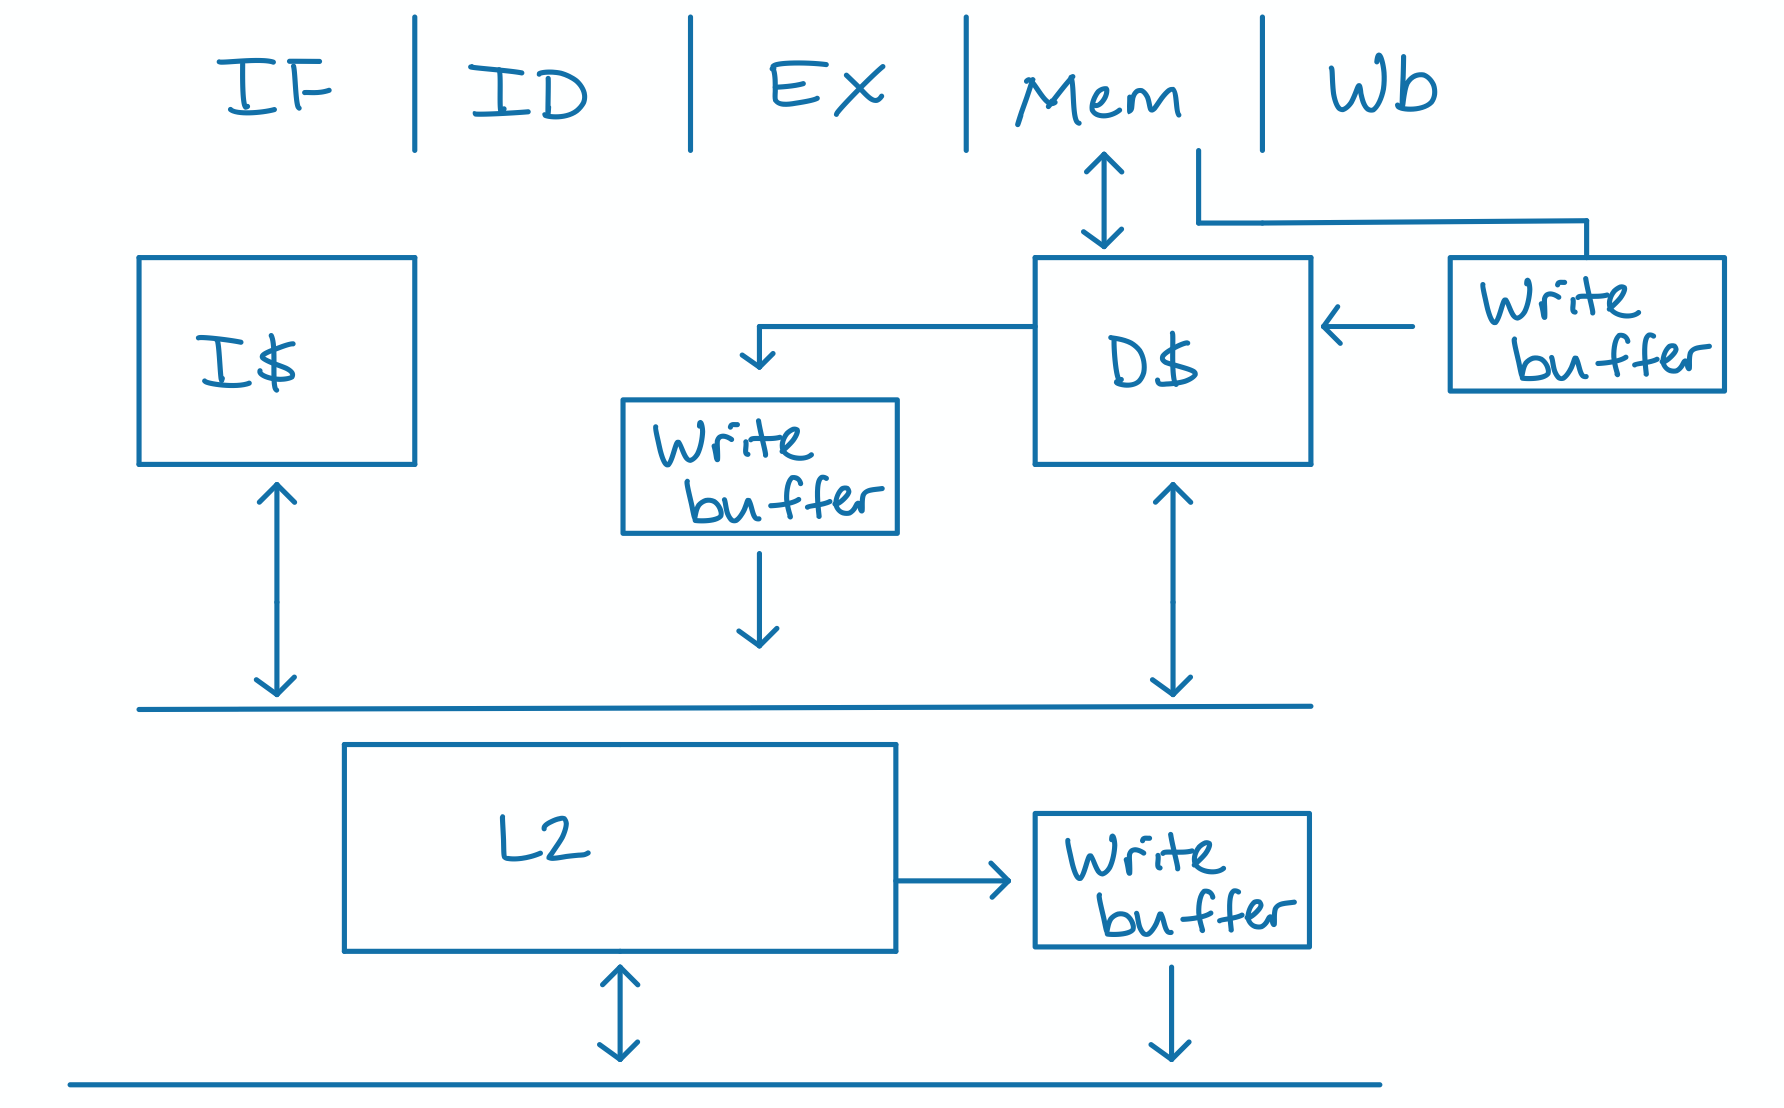
\includegraphics[width=0.80\textwidth]{Screen Shot 2020-05-15 at 00.44.40.png}
        \caption{Write Buffer for Question 5e}
        \label{fig:WriteBuffer}
        \end{figure}

        \item Describe each of the following architectures: Von Neumann, Harvard, Modified Harvard.\\[1em]
        Von Neumann architecture stores instructions and data in the same memory, while Harvard architecture stores instructions and data in separate memories. A modified Harvard architecture is where we go from a split cache at one level to a unified cache at the next level. This contrasts with a complete Harvard architecture where, at the programmer level, you split your instructions and data into separate memories.
    \end{enumerate}
\newpage
    \item \textbf{(15 points)} The following questions are related to virtual memory:
    \begin{enumerate}
        \item What was the primary reason virtual memory was developed?\\[1em]
        Virtual memory was developed to cope with small amounts of main memory, swapping data between disk and main memory automatically.\\

        \item What are other advantages virtual memory provides?\\[1em]
        Other advantages of virtual memory include:
        \begin{itemize}
            \item Allowing multiple processes to share resources easily
            \item Each process or program has its own virtual view of memory
            \item Protection between various processes and between processes and the OS\\
        \end{itemize}

        \item What is the purpose of the TLB? How do the TLB and L1 cache work together?\\[1em]
        Operating systems use some form of Least Recently Used (LRU) to determine what goes into physical memory versus disk. The translation lookaside buffer (TLB) acts as a small cache (typically fully associative) that stores the most recently used page table entries in order to speed things up. It is managed by the operating system. The TLB works with the L1 cache by mapping the virtual page number that translates to a physical address. In my mind, this scenario is like a NAT in networking, where we map local IP addresses to public-facing IP addresses.\\

        \item What role does the Operating System (OS) play when it comes to virtual memory? What additional hardware support is required to run an OS?\\[1em]
        The OS manages page tables and the TLB, which keeps track of address mapping. Storing pages on disk allows a program’s virtual address space to be larger than the machines physical address space. Additional hardware support required to run an OS include User and Kernel modes and address regions.
    \end{enumerate}
\newpage
    \item \textbf{(15 points)} Assuming a direct-mapped cache with a byte-address that is broken up such that bits 0-2 are for the byte offset, bits 3-5 are for the word offset, bits 6-14 are for the index, and bits 15-31 are for the tag, answer the following questions:
    \begin{enumerate}
        \item How large are the words in this machine?\\[1em]
        $2^{\mathrm{byte\ offset}}=2^3=8\mathrm{\ bytes}=64\mathrm{\ bits.}$\\

        \item How many words are in each cache block? How many bytes are in each cache block?\\[1em]
        $2^{\mathrm{word\ offset}}=2^3=8$ words in each cache block.\\ $8\mathrm{\ words} \times 8\mathrm{\ bytes}=64$ bytes in each cache block.\\

        \item How many cache blocks are in the cache? How many sets are in the cache?\\[1em]
        $2^{\mathrm{index}}=2^9=512$ sets in the cache, and because it is direct-mapped, there are also 512 blocks.\\

        \item How large is the data store of this cache?\\[1em]
        $512 \times 64 = 32$KiB\\

        \item How large is the tag store? Assume a \textit{valid} and \textit{dirty} bit are included with each tag.\\[1em]
        Each tag is 19 bits and there are 512 tags
        $\rightarrow 19\mathrm{\ bits} \times 512\mathrm{\ tags}=9728$ bits.\\

        \item If you were to modify the cache to be 4-way set associative (\textit{different from homework}) but keep the data store the same size, what size would the tag and index be? How large would the tag store be?\\[1em]
        The index would decrease by two bits while the tag would increase by two bits. Thus the index would be 8 bits and the tag would be 20 bits (including valid and dirty bits). The number of tags is the same because each block needs a tag. The tag store would be $20\mathrm{\ bits} \times 512\mathrm{\ tags}=10240$ bits.\\

        \item How much memory can the above machine address?\\[1em]
        The address is 32 bits in length so this machine can address 4GiB.
    \end{enumerate}
\end{enumerate}
\end{document}
